\chapter{INFORME PREVIO}

\section{Graficar las formas de onda de un rectificador 3p con 6 diodos con carga R-C}

Al igual como se observa en un rectificador monofasico con una salida conformada por una red RC como se muestra en la figura \ref{fig:salida-rc-monofasico} esta es de naturaleza pulsante debido al proceso de carga y descarga del capacitor.

% TODO: \usepackage{graphicx} required
\begin{figure}[h]
	\centering
	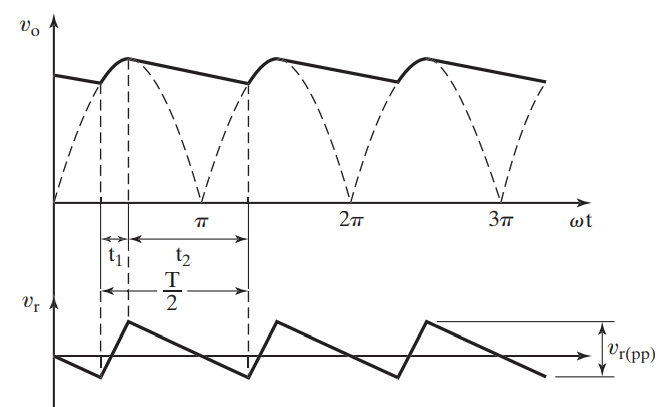
\includegraphics[width=0.7\linewidth]{media/salida-RC-monofasico}
	\caption{Forma de onda de un rectificador monofásico con carga RC}
	\label{fig:salida-rc-monofasico}
\end{figure}

En el rectificador trifásico para una carga de la misma naturaleza (RC) se vera un comportamiento o forma de onda similar, sin embargo debido a la presencia de cada línea la señal "pulsante" para este caso tendrá una forma casi continua, pudiendo dislumbrar tales puntos para pequeños instantes de tiempos como se muestra en la simulación \ref{fig:forma-onda-RC} de PSIM.

\begin{figure}[h]
	\centering
	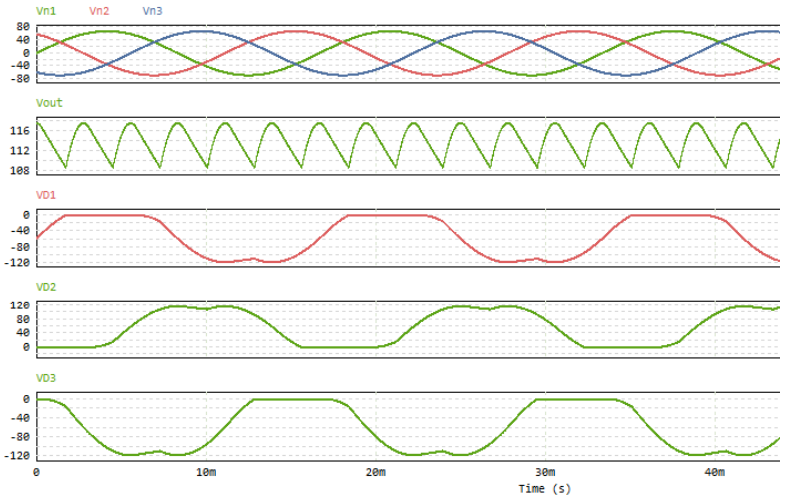
\includegraphics[width=0.7\linewidth]{media/forma-onda-RC}
	\caption{Forma de onda de salida para un rectificador trifasico con carga RC}
	\label{fig:forma-onda-RC}
\end{figure}
